\subsection{User interfaces}
Here we present the mock-ups of the application user interface.\\
We will present the user interface regarding only the two mobile applications (one for the Passengers and one for the Taxi Drivers).\\
The web application interface for the Passenger is a natural extension of the mobile one.
\subsubsection{Home page for the Passenger}
\begin{figure}[H]
\centering
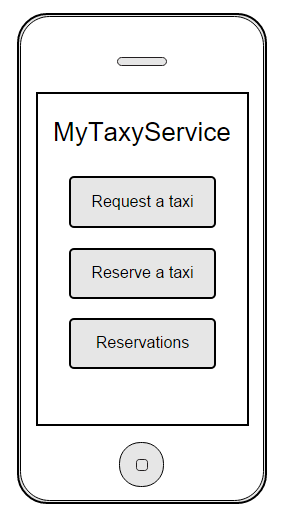
\includegraphics[scale=0.6]{Images/home_page}
\caption{Home page for the Passenger}
\end{figure}
This screen will present to the Passenger the possibility to 
\begin{itemize}
\item Request an immediate taxi service
\item Reserve a taxi for a future journey
\end{itemize}

\subsubsection{Request for an immediate taxi}
\begin{figure}[H]
\centering
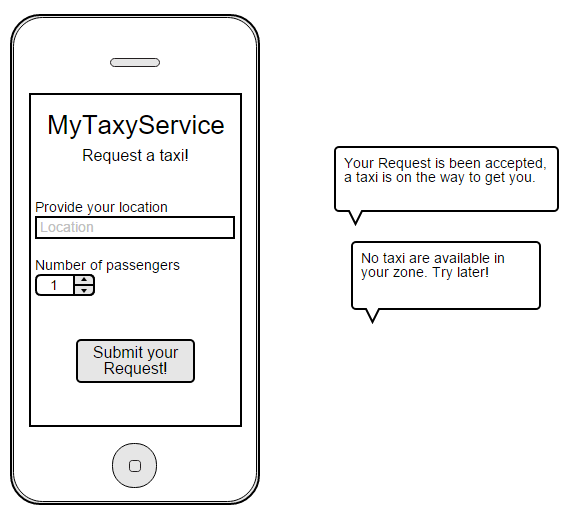
\includegraphics[scale=0.6]{Images/taxi_request}
\caption{Request for an immediate taxi}
\end{figure}
This screen is reached by pressing the button "REQUEST A TAXI" from the Home Page. The user can:
\begin{itemize}
\item Insert his location
\item The number of passengers of the requested ride
\item Submit the request
\end{itemize} 
If one or more necessary information is not inserted (missing) the user will be notified with an appropriate pop-up.


\subsubsection{Reservation of a taxi}
\begin{figure}[H]
\centering
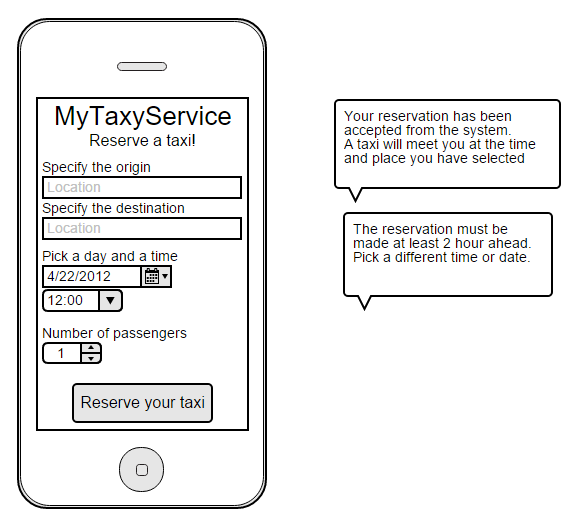
\includegraphics[scale=0.6]{Images/taxi_reservation}
\caption{Reservation of a taxi}
\end{figure}
This screen is reached by pressing the button "RESERVE A TAXI" from the Home Page. The user can:
\begin{itemize}
\item Specify his actual location
\item Specify the destination of the journey
\item Specify the date and hour of the meeting time
\item Specify the number of passengers
\item Submit the reservation request to the system
\end{itemize}
If one or more necessary information is not inserted (missing) the user will be notified with an appropriate pop-up.

\subsubsection{Acknowledgement of a taxi request/reservation to a Passenger}
\begin{figure}[H]
\centering
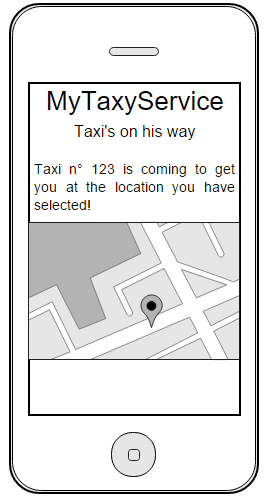
\includegraphics[scale=0.6]{Images/taxi_coming}
\caption{First screen of the application for Taxi Drivers}
\end{figure}
This screen is reached when a taxi is allocated to the Passenger request, both in case of immediate request and reservation.\\
The screen will present:
\begin{itemize}
\item Taxi identification number
\item Waiting time
\item Resume of the submitted data by the Passenger (meeting location, ecc...)
\end{itemize}

\subsubsection{Start working day for a Taxi Driver}
This is the first screen a Taxi Driver will see at the opening of the application:
\begin{figure}[H]
\centering
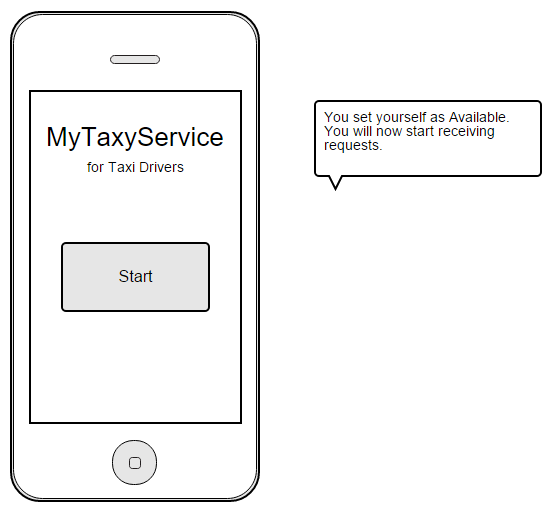
\includegraphics[scale=0.6]{Images/start_taxi_driver}
\caption{First screen of the application for Taxi Drivers}
\end{figure}

\subsubsection{Taxi Driver's waiting for a requests}
\begin{figure}[H]
\centering
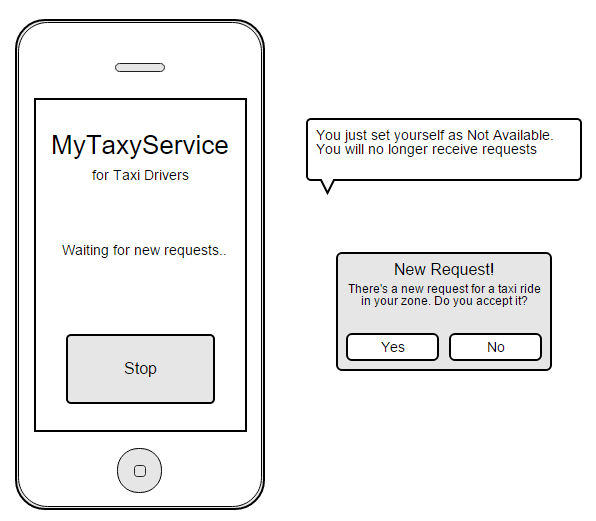
\includegraphics[scale=0.6]{Images/wait_taxi_driver}
\caption{Waiting screen for a taxi driver}
\end{figure}
This screen is reached by pressing on the "START" button on the previous screen.\\
Once a request is submitted to the taxi driver the application notifies him with a pop-up saying that there is a request for a ride in the current zone.\\
It is asked to the taxi driver if he wants to accept the request or not.

\subsubsection{Communication of the location to a Taxi Driver}
\begin{figure}[H]
\centering
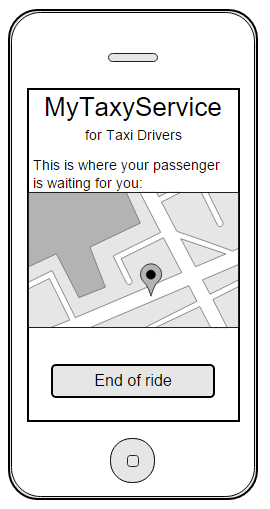
\includegraphics[scale=0.6]{Images/taxi_driver_busy}
\caption{Communication of the Passenger location to the Taxi Driver}
\end{figure}
This screen is reached by pressing the "YES" button on the pop-up displayed on the previous screen. It will be present a map indicating the position of the Passenger (meeting location). When the ride will be done the Taxi Driver will press the "END OF RIDE" button to notify his availability.


\subsection{GUI state chart}
We can summarize the behavior of the user interface through a state chart in which every state represents a specific screen of the application and each transition is basically a user input or a system communication to the application.
\subsubsection{Taxi driver usage of the user interface}
\begin{figure}[H]
\centering
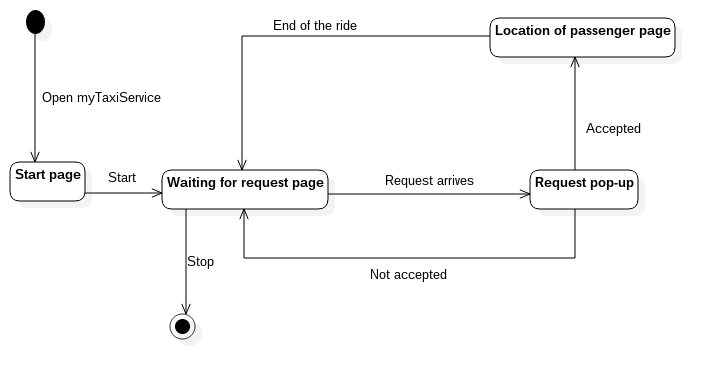
\includegraphics[scale=0.6]{Images/statechart_GUI}
\caption{Communication of the Passenger location to the Taxi Driver}
\end{figure}